% Hur är sensorenheten designad?

\section{Sensorenhet}

Sensorenheten har till uppgift att förse huvudenheten med sensordata. Sensordatan den returnerar är obehandlad rådata.

\subsection{Hårdvara}

\begin{figure}[h!]
	\centering
	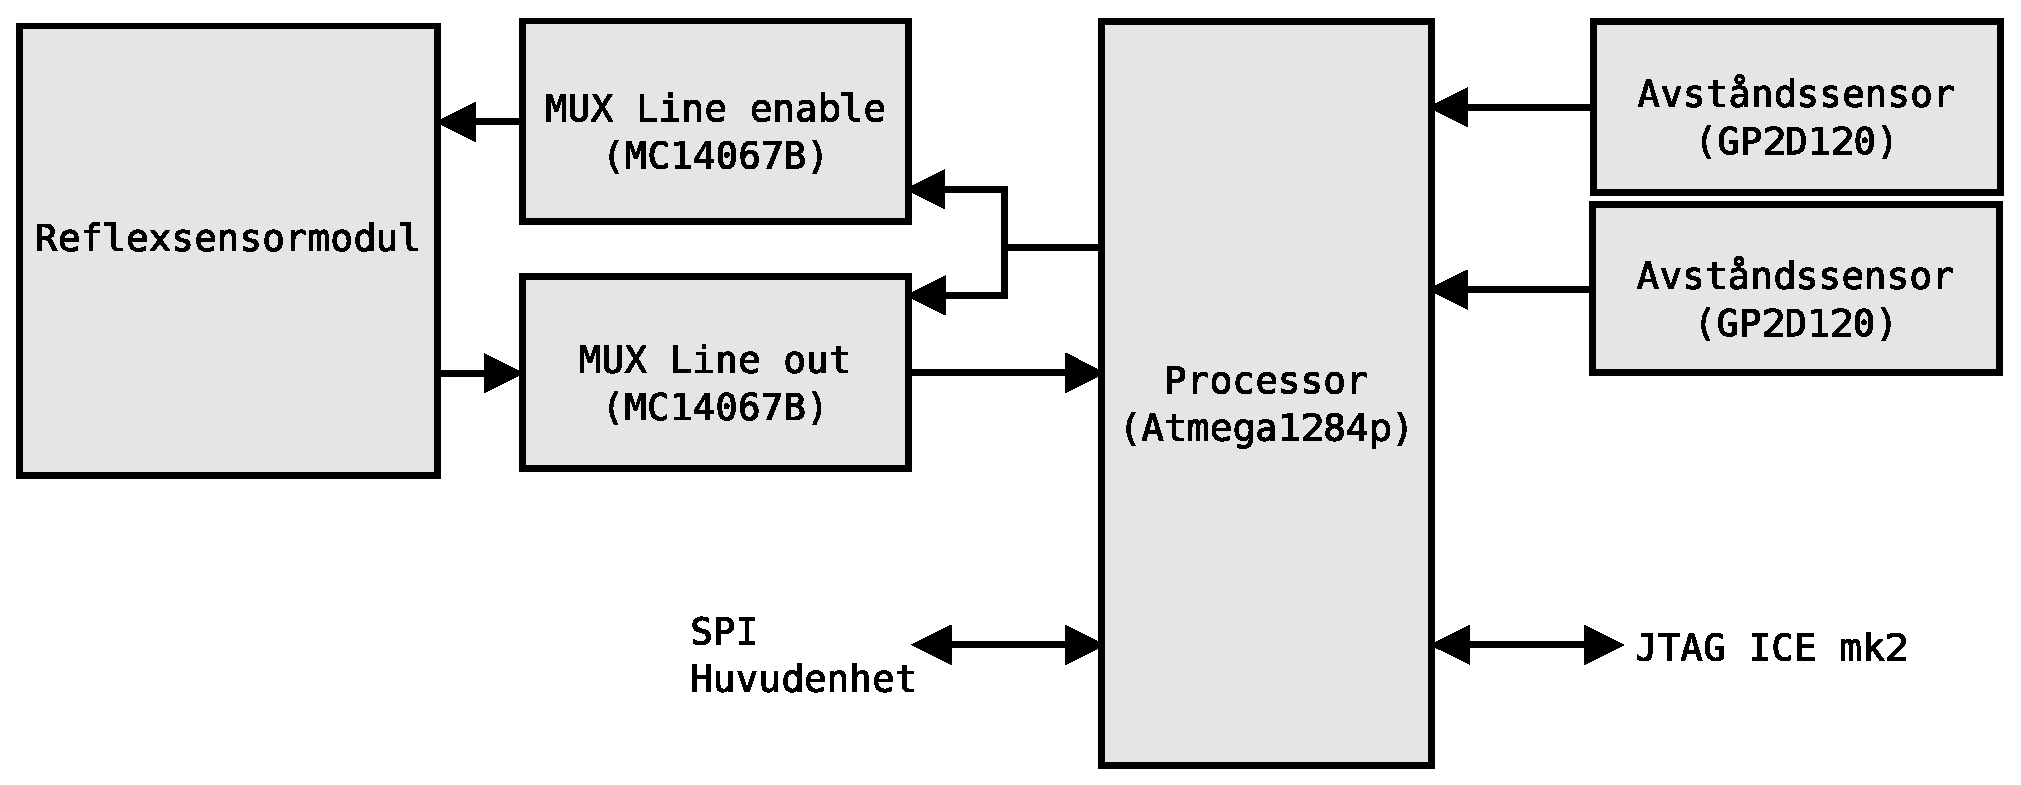
\includegraphics[scale=0.4]{grafik/sensorenhet-oversikt}
	\caption{Översikt av sensorenheten }
\end{figure}

Sensorenheten består av en Atmega1284p, en reflexsensormodul och två avståndssensorer. Reflexsensormodulen är kopplad via två 16-1 muxar till enkretsdatorn. Den ena muxen används för att styra en enable-signal till rätt reflexsensor och den andra för att välja rätt utsignal. Enkretsdatorn är ansluten till huvudenheten med en \todo{20lol-pinnarskabel?} över vilken de kommunicerar via SPI.

\begin{figure}[h!]
	\centering
	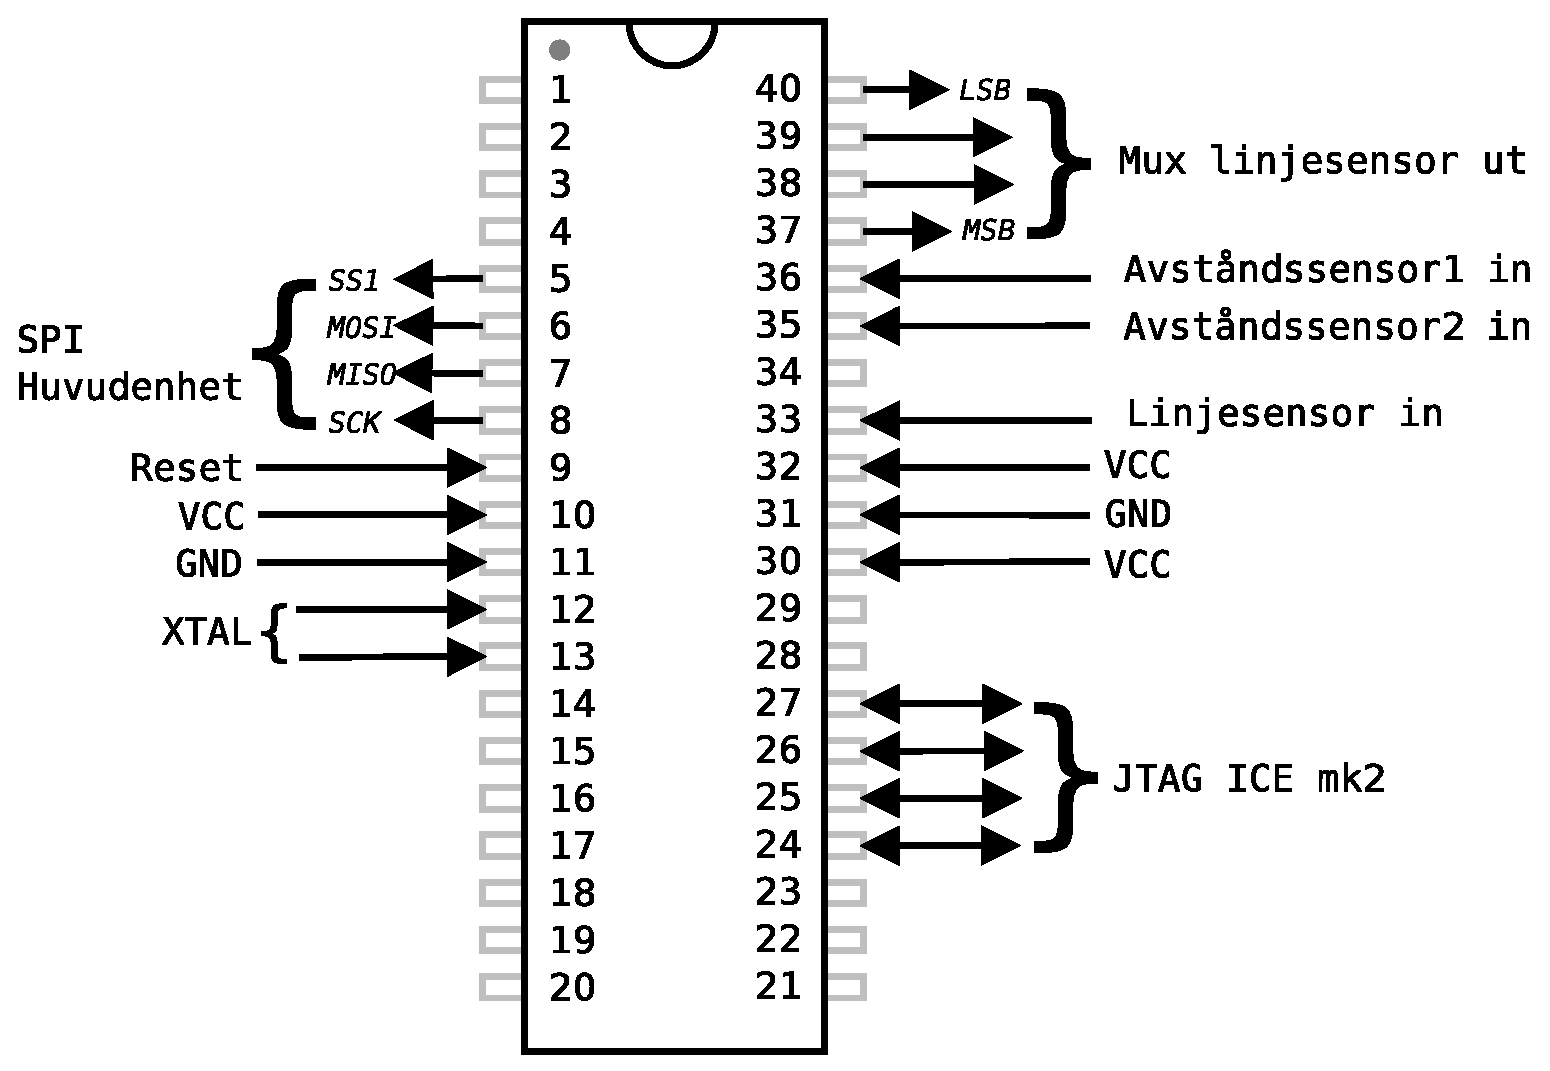
\includegraphics[scale=0.5]{grafik/sensorenhet-processor}
	\caption{Schema över hur enkretssdatorn i sensorenheten är ansluten till övrig hårdvara.}
\end{figure}

\subsubsection{Reflexsensormodul}

Reflexsensormodulens syfte är att detektera banan längs vilken roboten skall röra sig. Den består av 11 reflexsensorer som i sig består av en IR-diod och en fototransistor. Utsignalen ligger mellan 0V och 5V. De ger låg utspänning då underlaget reflekterar mycket ljus, och hög utspänning då lite ljus reflekteras.

\subsubsection{Avståndssensorer}

Avståndssensorerna är av typen GP2D120 vilken använder ljus för att detektera avståndet. Dess utsignal är en analog spänning mellan 0V och 3.2V.

\subsection{Mjukvara}

All mjukvara på sensorenheten är skriven i $C$ och finns på enkretsdatorn. Den består av två delar, illustrerat i figur \ref{sensorenhet-mjukvara}.

\begin{figure}[h!]
	\centering
	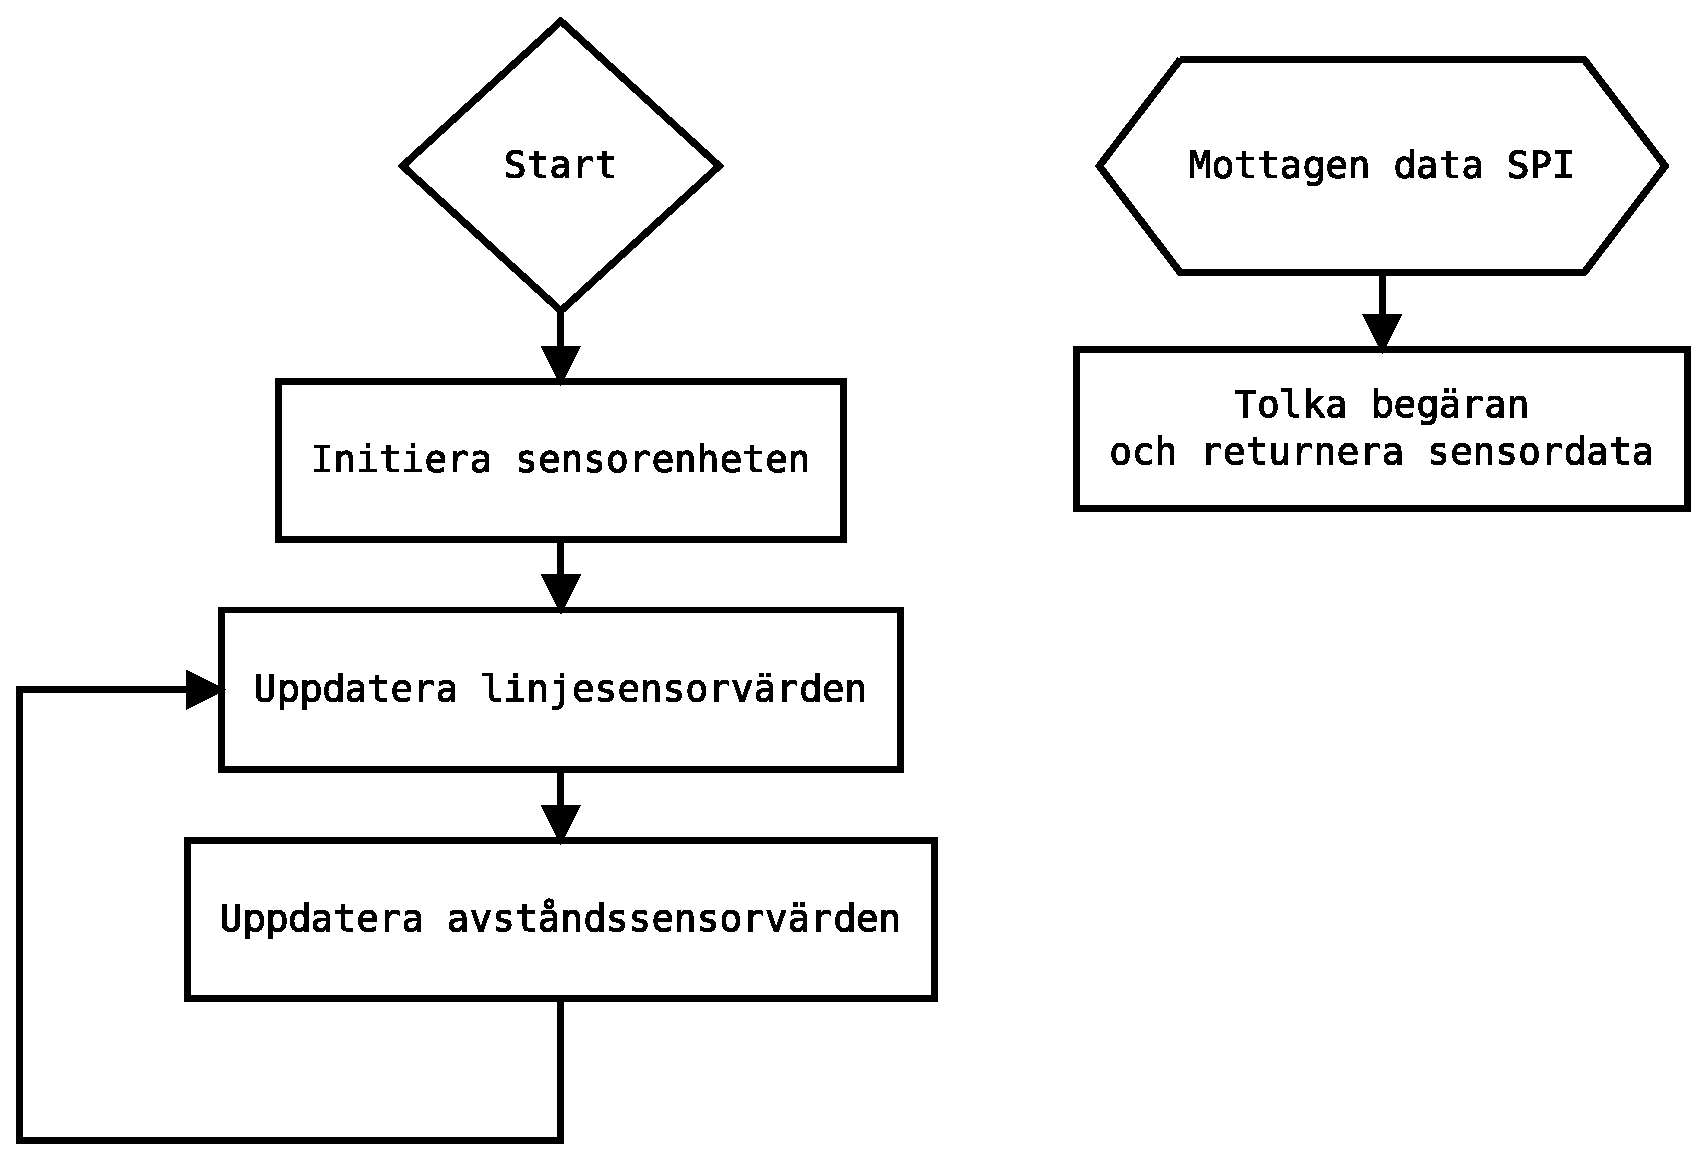
\includegraphics[scale=0.4]{grafik/sensorenhet-mjukvara}
	\caption{Till vänster sensorenhetens \todo{huvudslinga}, till höger den avbrottsrutin som körs vid mottagen data över SPI.} \label{sensorenhet-mjukvara}
\end{figure}

För det första körs en mainloop där sensordata kontinuerligt uppdateras. Först itererar vi igenom Reflexsensorerna genom att först styra om enable-signalen till den aktuella sensorn och därefter utföra en AD-omvandling på den signal vi får tillbaks och sedan gå till nästa. Därefter utför vi i tur och ordning en AD-omvandling på insignalerna från avståndssensorerna. Alla värden sparas i en global datastruktur.
\newline
För det andra tar sensorenheten emot begäran om sensordata från huvudenheten över SPI. När en sådan förfrågan inkommer triggas ett avbrott i vilket sensorenheten svarar med det aktuella sensorvärdet. Då inget i avläsningen av sensorerna är tidskritiskt behöver vi inte oroa oss för när dessa avbrott kommer.
